\documentclass[tikz,border=10pt]{standalone}
\usetikzlibrary{arrows.meta, calc, patterns}

\begin{document}
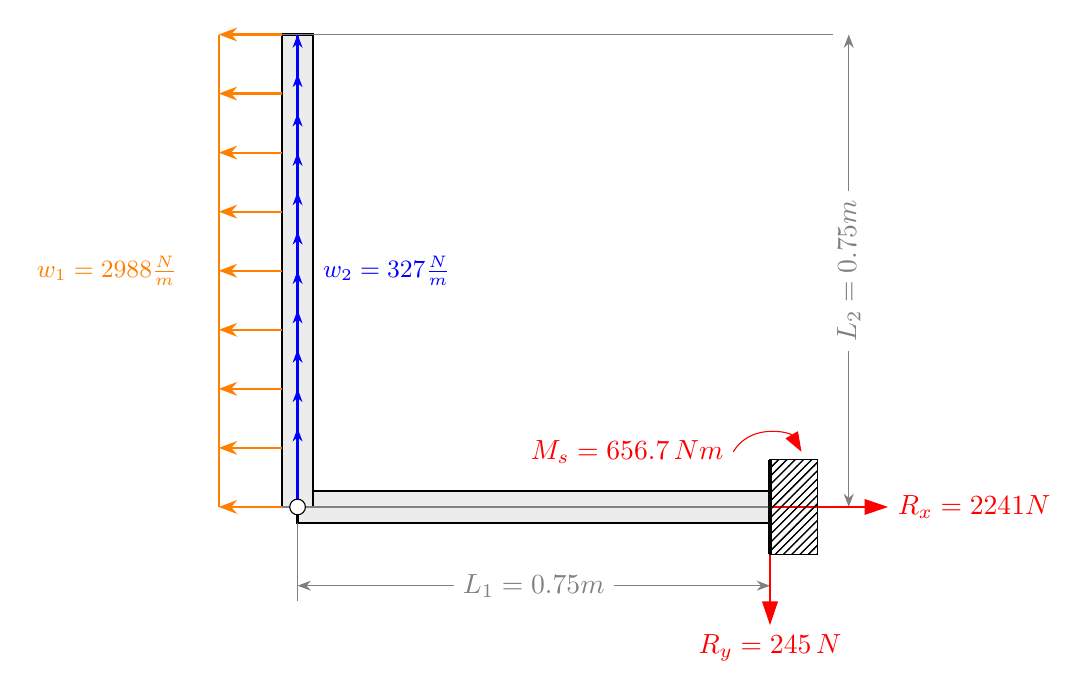
\begin{tikzpicture}[
    force/.style={- {Stealth[scale=1.2]}, red, thick},
    reaction/.style={- {Stealth[scale=1.2]}, blue!70!black, thick},
    beam/.style={draw=black, fill=gray!15, thick},
    joint/.style={circle, draw=black, fill=white, inner sep=2pt},
    ext/.style={gray, thin},
    dim/.style={<->, >=Stealth, gray, thin}
]

    % --- Parameters ---
    \def\L{6}           % Visual length
    \def\width{0.4}     % Beam thickness
    \def\loadL{4.5}     % Length of the distributed load
    \def\arrowgap{0.6}  % Number of arrows in the load

    % --- Coordinates ---
    \coordinate (Shoulder) at (0,0);
    \coordinate (Elbow) at (-\L, 0);
    \coordinate (Wrist) at (-\L, \L);

    % --- Draw Support (Fixed Shoulder) ---
    \draw[pattern=north east lines, draw=black] (0,-0.6) rectangle (0.6,0.6);
    \draw[ultra thick] (0,-0.6) -- (0,0.6);

    % --- Draw Beams ---
    \draw[beam] (-\L, -\width/2) rectangle (0, \width/2); % Beam 1
    \draw[beam] ({-\L-\width/2}, 0) rectangle ({-\L+\width/2}, \L); % Beam 2

    % --- Dimensioning for Beam 1 (Horizontal) ---
    \def\offH{-1} % Offset below the beam
    \draw[ext] (-\L, -\width/2) -- (-\L, \offH - 0.2); % Left extension
    \draw[ext] (0, -\width/2) -- (0, \offH - 0.2);      % Right extension
    \draw[dim] (-\L, \offH) -- (0, \offH) 
        node[midway, fill=white] {$L_1 = 0.75\text{m}$};

    % --- Dimensioning for Beam 2 (Vertical) ---
    % Placed further to the left to avoid your friction load
    \def\offV{7} 
    \draw[ext] ({-\L-\width/2}, 0) -- ({-\L+\offV-0.2}, 0); % Bottom extension
    \draw[ext] ({-\L-\width/2}, \L) -- ({-\L+\offV-0.2}, \L); % Top extension
    \draw[dim] ({-\L+\offV}, 0) -- ({-\L+\offV}, \L) 
        node[midway, fill=white, rotate=90] {$L_2 = 0.75\text{m}$};
        
    % --- Reaction Forces (Shoulder) ---
    % Placed clearly with arrows
    \draw [red, -{Triangle[length=3mm, width=2mm]}] (0,0) -- (1.5, 0) node[right] {$R_x = 2241 \text{N}$};
    \draw [red, -{Triangle[length=3mm, width=2mm]}] (0,0) -- (0, -1.5) node[below] {$R_y=245 \,\text{N}$};
    % Moment reaction (since it's a fixed support)
        \draw[red, {Triangle[length=2.5mm, width=1.8mm]-}] (0.4, 0.7) arc (30:150:0.5) node[left] {$M_s=656.7 \, \text{Nm}$};
    
    % --- Distributed Friction Load (Downward) ---
    % Vertical line to the left of Beam 2
    \draw[blue, thick] ({-\L}, 0) -- ({-\L}, {\L});
    \foreach \x in {0, 0.5, ..., 5} {
    \draw[blue, Stealth-] (-\L,\L-\x) -- (-\L, \L-\x-0.5);
  }
    % Label for the blue friction load positioned to the right
    \node[right, blue, font=\small, align=left] at (-\L + 0.2, \L/2) {
        $w_2 = 327 \frac{\text{N}}{\text{m}}$
    };
   % --- Distributed Normal Load (Horizontal/Perpendicular) ---
    % For a vertical beam, the normal load acts horizontally. 
    % --- Distributed Normal Load (Horizontal/Perpendicular) ---
    % Arrows now start at the beam surface and point left toward the boundary line
    \def\normL{6}      % Length of the load distribution
    \def\normX{-1}   % Horizontal offset for the load line
    
    % Boundary line for the normal load (the "tips" of the arrows)
    \draw[orange, thick] ({-\L+\normX}, \L) -- ({-\L+\normX}, {\L-\normL});
    
    % Horizontal arrows pointing LEFT
    \foreach \y in {0, 0.75, ..., \normL} {
        \draw[orange, -Stealth, thick] ({-\L-\width/2}, {\L-\y}) -- ({-\L+\normX}, {\L-\y});
    }
    
    % Label for Normal Load (moved slightly further left to avoid arrow overlap)
    \node[left, orange, font=\small, align=right] at ({-\L+\normX-0.3}, {\L-\normL/2}) {
        $w_1=2988 \frac{\text{N}}{\text{m}}$  
    };
   
    % --- Draw Support (Fixed Shoulder) ---
    \draw[pattern=north east lines, draw=black] (0,-0.6) rectangle (0.6,0.6);
    \draw[ultra thick] (0,-0.6) -- (0,0.6);

    \node[joint] at (Elbow) {};
\end{tikzpicture}
\end{document}
